%\begin{frame}
%\frametitle{Nonlinearity of Shapes}
%\begin{columns}[c]
%\column{0.7\textwidth}
%According to David Mumford (Fields Medal, 1974):
%\begin{quote}
%``Shapes are the ultimate non-linear sort of thing''
%\end{quote}
%
%Relative shapes can not be added and subtracted (ie, they are nonlinear).
%Instead, deformations should combined by composing them together.
%
%Deformations that are smooth and invertible are known as \emph{diffeomorphisms}, and form a mathematical \emph{group}.
%
%\column{0.3\textwidth}
%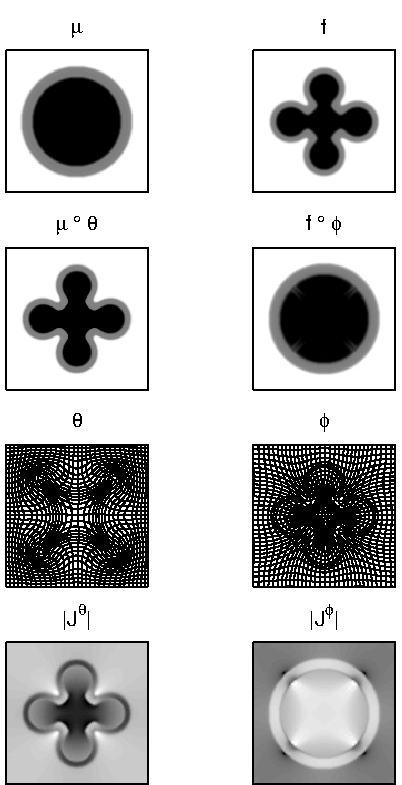
\includegraphics[height=.8\textheight]{2Dpics}
%\end{columns}
%\end{frame}

